\documentclass[11pt]{book}

\usepackage{amsmath}
\usepackage{amsthm}
\usepackage{circus}
% NOTE: parts of this have been altered from stock to:
% a) sidestep some issues with other packages etc. that this manual uses;
% b) make some formatting tweaks.
%
% Naturally, the result is CC BY-NC-SA 3.0 licenced.

%%%%%%%%%%%%%%%%%%%%%%%%%%%%%%%%%%%%%%%%%
% The Legrand Orange Book
% Structural Definitions File
% Version 2.1 (26/09/2018)
%
% Original author:
% Mathias Legrand (legrand.mathias@gmail.com) with modifications by:
% Vel (vel@latextemplates.com)
% 
% This file was downloaded from:
% http://www.LaTeXTemplates.com
%
% License:
% CC BY-NC-SA 3.0 (http://creativecommons.org/licenses/by-nc-sa/3.0/)
%
%%%%%%%%%%%%%%%%%%%%%%%%%%%%%%%%%%%%%%%%%

%----------------------------------------------------------------------------------------
%	VARIOUS REQUIRED PACKAGES AND CONFIGURATIONS
%----------------------------------------------------------------------------------------

\usepackage{graphicx} % Required for including pictures
\graphicspath{{Pictures/}} % Specifies the directory where pictures are stored

\usepackage{lipsum} % Inserts dummy text

\usepackage{tikz} % Required for drawing custom shapes

\usepackage[english]{babel} % English language/hyphenation

\usepackage{enumitem} % Customize lists
\setlist{nolistsep} % Reduce spacing between bullet points and numbered lists

\usepackage{booktabs} % Required for nicer horizontal rules in tables

\usepackage{xcolor} % Required for specifying colors by name
\definecolor{ocre}{RGB}{145,95,109} % Define the mauve color used for highlighting throughout the book

%----------------------------------------------------------------------------------------
%	MARGINS
%----------------------------------------------------------------------------------------

\usepackage{geometry} % Required for adjusting page dimensions and margins

\geometry{
	paper=a4paper, % Paper size, change to letterpaper for US letter size
	top=3cm, % Top margin
	bottom=3cm, % Bottom margin
	left=3cm, % Left margin
	right=3cm, % Right margin
	headheight=14pt, % Header height
	footskip=1.4cm, % Space from the bottom margin to the baseline of the footer
	headsep=10pt, % Space from the top margin to the baseline of the header
	%showframe, % Uncomment to show how the type block is set on the page
}

%----------------------------------------------------------------------------------------
%	FONTS
%----------------------------------------------------------------------------------------

%\usepackage{avant} % Use the Avantgarde font for headings
%\usepackage{times} % Use the Times font for headings
%\usepackage{mathptmx} % Use the Adobe Times Roman as the default text font together with math symbols from the Sym­bol, Chancery and Com­puter Modern fonts
\usepackage{stix}
\usepackage{tgtermes}
% while we don't technically need to load Heros here (we only use it for
% \metarefs), we do so to make sure it gets scaled.
\usepackage[scale=0.88]{tgheros}
\usepackage[scale=0.88]{tgadventor}
\usepackage[scaled]{beramono}

\usepackage{microtype} % Slightly tweak font spacing for aesthetics
\usepackage[utf8]{inputenc} % Required for including letters with accents
\usepackage[T1]{fontenc} % Use 8-bit encoding that has 256 glyphs

%----------------------------------------------------------------------------------------
%	BIBLIOGRAPHY AND INDEX
%----------------------------------------------------------------------------------------

\usepackage[style=numeric,citestyle=numeric,sorting=nyt,sortcites=true,autopunct=true,babel=hyphen,hyperref=true,abbreviate=false,backref=true,backend=biber]{biblatex}
\addbibresource{robocert.bib} % BibTeX bibliography file
\defbibheading{bibempty}{}

\usepackage{calc} % For simpler calculation - used for spacing the index letter headings correctly
\usepackage{makeidx} % Required to make an index
\makeindex % Tells LaTeX to create the files required for indexing

%----------------------------------------------------------------------------------------
%	MAIN TABLE OF CONTENTS
%----------------------------------------------------------------------------------------

\usepackage{titletoc} % Required for manipulating the table of contents

\contentsmargin{0cm} % Removes the default margin

% Part text styling (this is mostly taken care of in the PART HEADINGS section of this file)
\titlecontents{part}
	[0cm] % Left indentation
	{\addvspace{20pt}\bfseries} % Spacing and font options for parts
	{}
	{}
	{}

% Chapter text styling
\titlecontents{chapter}
	[1.25cm] % Left indentation
	{\addvspace{12pt}\large\sffamily\bfseries} % Spacing and font options for chapters
	{\color{ocre!60}\contentslabel[\Large\thecontentslabel]{1.25cm}\color{ocre}} % Formatting of numbered sections of this type
	{\color{ocre}} % Formatting of numberless sections of this type
	{\color{ocre!60}\normalsize\;\titlerule*[.5pc]{.}\;\thecontentspage} % Formatting of the filler to the right of the heading and the page number

% Section text styling
\titlecontents{section}
	[1.25cm] % Left indentation
	{\addvspace{3pt}\sffamily\bfseries} % Spacing and font options for sections
	{\contentslabel[\thecontentslabel]{1.25cm}} % Formatting of numbered sections of this type
	{} % Formatting of numberless sections of this type
	{\hfill\color{black}\thecontentspage} % Formatting of the filler to the right of the heading and the page number

% Subsection text styling
\titlecontents{subsection}
	[1.25cm] % Left indentation
	{\addvspace{1pt}\sffamily\small} % Spacing and font options for subsections
	{\contentslabel[\thecontentslabel]{1.25cm}} % Formatting of numbered sections of this type
	{} % Formatting of numberless sections of this type
	{\ \titlerule*[.5pc]{.}\;\thecontentspage} % Formatting of the filler to the right of the heading and the page number

% Figure text styling
\titlecontents{figure}
	[1.25cm] % Left indentation
	{\addvspace{1pt}\sffamily\small} % Spacing and font options for figures
	{\thecontentslabel\hspace*{1em}} % Formatting of numbered sections of this type
	{} % Formatting of numberless sections of this type
	{\ \titlerule*[.5pc]{.}\;\thecontentspage} % Formatting of the filler to the right of the heading and the page number

% Table text styling
\titlecontents{table}
	[1.25cm] % Left indentation
	{\addvspace{1pt}\sffamily\small} % Spacing and font options for tables
	{\thecontentslabel\hspace*{1em}} % Formatting of numbered sections of this type
	{} % Formatting of numberless sections of this type
	{\ \titlerule*[.5pc]{.}\;\thecontentspage} % Formatting of the filler to the right of the heading and the page number

%----------------------------------------------------------------------------------------
%	MINI TABLE OF CONTENTS IN PART HEADS
%----------------------------------------------------------------------------------------

% Chapter text styling
\titlecontents{lchapter}
	[0em] % Left indentation
	{\addvspace{15pt}\large\sffamily\bfseries} % Spacing and font options for chapters
	{\color{ocre}\contentslabel[\Large\thecontentslabel]{1.25cm}\color{ocre}} % Chapter number
	{}  
	{\color{ocre}\normalsize\sffamily\bfseries\;\titlerule*[.5pc]{.}\;\thecontentspage} % Page number

% Section text styling
\titlecontents{lsection}
	[0em] % Left indentation
	{\sffamily\small} % Spacing and font options for sections
	{\contentslabel[\thecontentslabel]{1.25cm}} % Section number
	{}
	{}

% Subsection text styling (note these aren't shown by default, display them by searchings this file for tocdepth and reading the commented text)
\titlecontents{lsubsection}
	[.5em] % Left indentation
	{\sffamily\footnotesize} % Spacing and font options for subsections
	{\contentslabel[\thecontentslabel]{1.25cm}}
	{}
	{}

%----------------------------------------------------------------------------------------
%	HEADERS AND FOOTERS
%----------------------------------------------------------------------------------------

\usepackage{fancyhdr} % Required for header and footer configuration

\pagestyle{fancy} % Enable the custom headers and footers

\renewcommand{\chaptermark}[1]{\markboth{\sffamily\normalsize\bfseries\chaptername\ \thechapter.\ #1}{}} % Styling for the current chapter in the header
\renewcommand{\sectionmark}[1]{\markright{\sffamily\normalsize\thesection\hspace{5pt}#1}{}} % Styling for the current section in the header

\fancyhf{} % Clear default headers and footers
\fancyhead[LE,RO]{\sffamily\normalsize\thepage} % Styling for the page number in the header
\fancyhead[LO]{\rightmark} % Print the nearest section name on the left side of odd pages
\fancyhead[RE]{\leftmark} % Print the current chapter name on the right side of even pages
%\fancyfoot[C]{\thepage} % Uncomment to include a footer

\renewcommand{\headrulewidth}{0.5pt} % Thickness of the rule under the header

\fancypagestyle{plain}{% Style for when a plain pagestyle is specified
	\fancyhead{}\renewcommand{\headrulewidth}{0pt}%
}

% Removes the header from odd empty pages at the end of chapters
\makeatletter
\renewcommand{\cleardoublepage}{
\clearpage\ifodd\c@page\else
\hbox{}
\vspace*{\fill}
\thispagestyle{empty}
\newpage
\fi}

%----------------------------------------------------------------------------------------
%	THEOREM STYLES
%----------------------------------------------------------------------------------------

% v-- MattWindsor91: had to comment this out to get circus.sty to play nicely.
%\usepackage{amsmath,amsfonts,amssymb,amsthm} % For math equations, theorems, symbols, etc

\newcommand{\intoo}[2]{\mathopen{]}#1\,;#2\mathclose{[}}
\newcommand{\ud}{\mathop{\mathrm{{}d}}\mathopen{}}
\newcommand{\intff}[2]{\mathopen{[}#1\,;#2\mathclose{]}}
\renewcommand{\qedsymbol}{$\blacksquare$}
\newtheorem{notation}{Notation}[chapter]

% Boxed/framed environments
\newtheoremstyle{ocrenumbox}% Theorem style name
{0pt}% Space above
{0pt}% Space below
{\normalfont}% Body font
{}% Indent amount
{\small\bf\sffamily\color{ocre}}% Theorem head font
{\;}% Punctuation after theorem head
{0.25em}% Space after theorem head
{\small\sffamily\color{ocre}\thmname{#1}\nobreakspace\thmnumber{\@ifnotempty{#1}{}\@upn{#2}}% Theorem text (e.g. Theorem 2.1)
\thmnote{\nobreakspace\the\thm@notefont\sffamily\bfseries\color{black}---\nobreakspace#3.}} % Optional theorem note

\newtheoremstyle{blacknumex}% Theorem style name
{5pt}% Space above
{5pt}% Space below
{\normalfont}% Body font
{} % Indent amount
{\small\bf\sffamily}% Theorem head font
{\;}% Punctuation after theorem head
{0.25em}% Space after theorem head
{\small\sffamily{\tiny\ensuremath{\blacksquare}}\nobreakspace\thmname{#1}\nobreakspace\thmnumber{\@ifnotempty{#1}{}\@upn{#2}}% Theorem text (e.g. Theorem 2.1)
\thmnote{\nobreakspace\the\thm@notefont\sffamily\bfseries---\nobreakspace#3.}}% Optional theorem note

\newtheoremstyle{blacknumbox} % Theorem style name
{0pt}% Space above
{0pt}% Space below
{\normalfont}% Body font
{}% Indent amount
{\small\bf\sffamily}% Theorem head font
{\;}% Punctuation after theorem head
{0.25em}% Space after theorem head
{\small\sffamily\thmname{#1}\nobreakspace\thmnumber{\@ifnotempty{#1}{}\@upn{#2}}% Theorem text (e.g. Theorem 2.1)
\thmnote{\nobreakspace\the\thm@notefont\sffamily\bfseries---\nobreakspace#3.}}% Optional theorem note

% Non-boxed/non-framed environments
\newtheoremstyle{ocrenum}% Theorem style name
{5pt}% Space above
{5pt}% Space below
{\normalfont}% Body font
{}% Indent amount
{\small\bf\sffamily\color{ocre}}% Theorem head font
{\;}% Punctuation after theorem head
{0.25em}% Space after theorem head
{\small\sffamily\color{ocre}\thmname{#1}\nobreakspace\thmnumber{\@ifnotempty{#1}{}\@upn{#2}}% Theorem text (e.g. Theorem 2.1)
\thmnote{\nobreakspace\the\thm@notefont\sffamily\bfseries\color{black}---\nobreakspace#3.}} % Optional theorem note
\makeatother

% Defines the theorem text style for each type of theorem to one of the three styles above
\newcounter{dummy} 
\numberwithin{dummy}{section}
\theoremstyle{ocrenumbox}
\newtheorem{theoremeT}[dummy]{Theorem}
\newtheorem{problem}{Problem}[chapter]
\newtheorem{exerciseT}{Exercise}[chapter]
\theoremstyle{blacknumex}
\newtheorem{exampleT}{Example}[chapter]
\theoremstyle{blacknumbox}
\newtheorem{vocabulary}{Vocabulary}[chapter]
\newtheorem{definitionT}{Definition}[section]
\newtheorem{corollaryT}[dummy]{Corollary}
\theoremstyle{ocrenum}
\newtheorem{proposition}[dummy]{Proposition}

%----------------------------------------------------------------------------------------
%	DEFINITION OF COLORED BOXES
%----------------------------------------------------------------------------------------

\RequirePackage[framemethod=default]{mdframed} % Required for creating the theorem, definition, exercise and corollary boxes

% Theorem box
\newmdenv[skipabove=7pt,
skipbelow=7pt,
backgroundcolor=black!5,
linecolor=ocre,
innerleftmargin=5pt,
innerrightmargin=5pt,
innertopmargin=5pt,
leftmargin=0cm,
rightmargin=0cm,
innerbottommargin=5pt]{tBox}

% Exercise box	  
\newmdenv[skipabove=7pt,
skipbelow=7pt,
rightline=false,
leftline=true,
topline=false,
bottomline=false,
backgroundcolor=ocre!10,
linecolor=ocre,
innerleftmargin=5pt,
innerrightmargin=5pt,
innertopmargin=5pt,
innerbottommargin=5pt,
leftmargin=0cm,
rightmargin=0cm,
linewidth=4pt]{eBox}	

% Definition box
\newmdenv[skipabove=7pt,
skipbelow=7pt,
rightline=false,
leftline=true,
topline=false,
bottomline=false,
linecolor=ocre,
innerleftmargin=5pt,
innerrightmargin=5pt,
innertopmargin=0pt,
leftmargin=0cm,
rightmargin=0cm,
linewidth=4pt,
innerbottommargin=0pt]{dBox}	

% Corollary box
\newmdenv[skipabove=7pt,
skipbelow=7pt,
rightline=false,
leftline=true,
topline=false,
bottomline=false,
linecolor=gray,
backgroundcolor=black!5,
innerleftmargin=5pt,
innerrightmargin=5pt,
innertopmargin=5pt,
leftmargin=0cm,
rightmargin=0cm,
linewidth=4pt,
innerbottommargin=5pt]{cBox}

% Creates an environment for each type of theorem and assigns it a theorem text style from the "Theorem Styles" section above and a colored box from above

\renewenvironment{theorem}{\begin{tBox}\begin{theoremeT}}{\end{theoremeT}\end{tBox}}
\newenvironment{exercise}{\begin{eBox}\begin{exerciseT}}{\hfill{\color{ocre}\tiny\ensuremath{\blacksquare}}\end{exerciseT}\end{eBox}}				  
\newenvironment{definition}{\begin{dBox}\begin{definitionT}}{\end{definitionT}\end{dBox}}	
\newenvironment{example}{\begin{exampleT}}{\hfill{\tiny\ensuremath{\blacksquare}}\end{exampleT}}		
\newenvironment{corollary}{\begin{cBox}\begin{corollaryT}}{\end{corollaryT}\end{cBox}}	

%----------------------------------------------------------------------------------------
%	REMARK ENVIRONMENT
%----------------------------------------------------------------------------------------

\newenvironment{remark}{\par\vspace{10pt}\small % Vertical white space above the remark and smaller font size
\begin{list}{}{
\leftmargin=35pt % Indentation on the left
\rightmargin=25pt}\item\ignorespaces % Indentation on the right
\makebox[-2.5pt]{\begin{tikzpicture}[overlay]
\node[draw=ocre!60,line width=1pt,circle,fill=ocre!25,font=\sffamily\bfseries,inner sep=2pt,outer sep=0pt] at (-15pt,0pt){\textcolor{ocre}{R}};\end{tikzpicture}} % Orange R in a circle
\advance\baselineskip -1pt}{\end{list}\vskip5pt} % Tighter line spacing and white space after remark

%----------------------------------------------------------------------------------------
%	SECTION NUMBERING IN THE MARGIN
%----------------------------------------------------------------------------------------

\makeatletter
\renewcommand{\@seccntformat}[1]{\llap{\textcolor{ocre}{\csname the#1\endcsname}\hspace{1em}}}                    
\renewcommand{\section}{\@startsection{section}{1}{\z@}
{-4ex \@plus -1ex \@minus -.4ex}
{1ex \@plus.2ex }
{\normalfont\large\sffamily\bfseries}}
\renewcommand{\subsection}{\@startsection {subsection}{2}{\z@}
{-3ex \@plus -0.1ex \@minus -.4ex}
{0.5ex \@plus.2ex }
{\normalfont\sffamily\bfseries}}
\renewcommand{\subsubsection}{\@startsection {subsubsection}{3}{\z@}
{-2ex \@plus -0.1ex \@minus -.2ex}
{.2ex \@plus.2ex }
{\normalfont\small\sffamily\bfseries}}                        
\renewcommand\paragraph{\@startsection{paragraph}{4}{\z@}
{-2ex \@plus-.2ex \@minus .2ex}
{.1ex}
{\normalfont\small\sffamily\bfseries}}

%----------------------------------------------------------------------------------------
%	PART HEADINGS
%----------------------------------------------------------------------------------------

% Numbered part in the table of contents
\newcommand{\@mypartnumtocformat}[2]{%
	\setlength\fboxsep{0pt}%
	\noindent\colorbox{ocre!20}{\strut\parbox[c][.7cm]{\ecart}{\color{ocre!70}\Large\sffamily\bfseries\centering#1}}\hskip\esp\colorbox{ocre!40}{\strut\parbox[c][.7cm]{\linewidth-\ecart-\esp}{\Large\sffamily\centering#2}}%
}

% Unnumbered part in the table of contents
\newcommand{\@myparttocformat}[1]{%
	\setlength\fboxsep{0pt}%
	\noindent\colorbox{ocre!40}{\strut\parbox[c][.7cm]{\linewidth}{\Large\sffamily\centering#1}}%
}

\newlength\esp
\setlength\esp{4pt}
\newlength\ecart
\setlength\ecart{1.2cm-\esp}
\newcommand{\thepartimage}{}%
\newcommand{\partimage}[1]{\renewcommand{\thepartimage}{#1}}%
\def\@part[#1]#2{%
\ifnum \c@secnumdepth >-2\relax%
\refstepcounter{part}%
\addcontentsline{toc}{part}{\texorpdfstring{\protect\@mypartnumtocformat{\thepart}{#1}}{\partname~\thepart\ ---\ #1}}
\else%
\addcontentsline{toc}{part}{\texorpdfstring{\protect\@myparttocformat{#1}}{#1}}%
\fi%
\startcontents%
\markboth{}{}%
{\thispagestyle{empty}%
\begin{tikzpicture}[remember picture,overlay]%
\node at (current page.north west){\begin{tikzpicture}[remember picture,overlay]%	
\fill[ocre!20](0cm,0cm) rectangle (\paperwidth,-\paperheight);
\node[anchor=north] at (4cm,-3.25cm){\color{ocre!40}\fontsize{220}{100}\sffamily\bfseries\thepart}; 
\node[anchor=south east] at (\paperwidth-1cm,-\paperheight+1cm){\parbox[t][][t]{8.5cm}{
\printcontents{l}{0}{\setcounter{tocdepth}{1}}% The depth to which the Part mini table of contents displays headings; 0 for chapters only, 1 for chapters and sections and 2 for chapters, sections and subsections
}};
\node[anchor=north east] at (\paperwidth-1.5cm,-3.25cm){\parbox[t][][t]{15cm}{\strut\raggedleft\color{ocre}\fontsize{30}{30}\sffamily\bfseries#2}};
\end{tikzpicture}};
\end{tikzpicture}}%
\@endpart}
\def\@spart#1{%
\startcontents%
\phantomsection
{\thispagestyle{empty}%
\begin{tikzpicture}[remember picture,overlay]%
\node at (current page.north west){\begin{tikzpicture}[remember picture,overlay]%	
\fill[ocre!20](0cm,0cm) rectangle (\paperwidth,-\paperheight);
\node[anchor=north east] at (\paperwidth-1.5cm,-3.25cm){\parbox[t][][t]{15cm}{\strut\raggedleft\color{ocre}\fontsize{30}{30}\sffamily\bfseries#1}};
\end{tikzpicture}};
\end{tikzpicture}}
\addcontentsline{toc}{part}{\texorpdfstring{%
\setlength\fboxsep{0pt}%
\noindent\protect\colorbox{ocre!40}{\strut\protect\parbox[c][.7cm]{\linewidth}{\Large\sffamily\protect\centering #1\quad\mbox{}}}}{#1}}%
\@endpart}
\def\@endpart{\vfil\newpage
\if@twoside
\if@openright
\null
\thispagestyle{empty}%
\newpage
\fi
\fi
\if@tempswa
\twocolumn
\fi}

%----------------------------------------------------------------------------------------
%	CHAPTER HEADINGS
%----------------------------------------------------------------------------------------

% A switch to conditionally include a picture, implemented by Christian Hupfer
\newif\ifusechapterimage
\usechapterimagetrue
\newcommand{\thechapterimage}{}%
\newcommand{\chapterimage}[1]{\ifusechapterimage\renewcommand{\thechapterimage}{#1}\fi}%
\newcommand{\autodot}{.}
\def\@makechapterhead#1{%
{\parindent \z@ \raggedright \normalfont
\ifnum \c@secnumdepth >\m@ne
\if@mainmatter
\begin{tikzpicture}[remember picture,overlay]
\node at (current page.north west)
{\begin{tikzpicture}[remember picture,overlay]
\node[anchor=north west,inner sep=0pt] at (0,0) {\ifusechapterimage\includegraphics[width=\paperwidth]{\thechapterimage}\fi};
\draw[anchor=west] (\Gm@lmargin,-9cm) node [line width=2pt,rounded corners=15pt,draw=ocre,fill=white,fill opacity=0.5,inner sep=15pt]{\strut\makebox[22cm]{}};
\draw[anchor=west] (\Gm@lmargin+.3cm,-9cm) node {\huge\sffamily\bfseries\color{black}\thechapter\autodot~#1\strut};
\end{tikzpicture}};
\end{tikzpicture}
\else
\begin{tikzpicture}[remember picture,overlay]
\node at (current page.north west)
{\begin{tikzpicture}[remember picture,overlay]
\node[anchor=north west,inner sep=0pt] at (0,0) {\ifusechapterimage\includegraphics[width=\paperwidth]{\thechapterimage}\fi};
\draw[anchor=west] (\Gm@lmargin,-9cm) node [line width=2pt,rounded corners=15pt,draw=ocre,fill=white,fill opacity=0.5,inner sep=15pt]{\strut\makebox[22cm]{}};
\draw[anchor=west] (\Gm@lmargin+.3cm,-9cm) node {\huge\sffamily\bfseries\color{black}#1\strut};
\end{tikzpicture}};
\end{tikzpicture}
\fi\fi\par\vspace*{270\p@}}}

%-------------------------------------------

\def\@makeschapterhead#1{%
\begin{tikzpicture}[remember picture,overlay]
\node at (current page.north west)
{\begin{tikzpicture}[remember picture,overlay]
\node[anchor=north west,inner sep=0pt] at (0,0) {\ifusechapterimage\includegraphics[width=\paperwidth]{\thechapterimage}\fi};
\draw[anchor=west] (\Gm@lmargin,-9cm) node [line width=2pt,rounded corners=15pt,draw=ocre,fill=white,fill opacity=0.5,inner sep=15pt]{\strut\makebox[22cm]{}};
\draw[anchor=west] (\Gm@lmargin+.3cm,-9cm) node {\huge\sffamily\bfseries\color{black}#1\strut};
\end{tikzpicture}};
\end{tikzpicture}
\par\vspace*{270\p@}}
\makeatother

%----------------------------------------------------------------------------------------
%	LINKS
%----------------------------------------------------------------------------------------

\usepackage{hyperref}
\hypersetup{hidelinks,backref=true,pagebackref=true,hyperindex=true,colorlinks=false,breaklinks=true,urlcolor=ocre,bookmarks=true,bookmarksopen=false}

\usepackage{bookmark}
\bookmarksetup{
open,
numbered,
addtohook={%
\ifnum\bookmarkget{level}=0 % chapter
\bookmarksetup{bold}%
\fi
\ifnum\bookmarkget{level}=-1 % part
\bookmarksetup{color=ocre,bold}%
\fi
}
}


\usepackage{braket} % set-builder notation
\usepackage{booktabs}
\usepackage{caption}
\usepackage{subcaption}
\usepackage{stmaryrd}

\usepackage{listings}

\usepackage{hyperref}
\usepackage{cleveref}

\usetikzlibrary{arrows.meta,matrix,positioning,quotes,shapes,calc,fit}
\colorlet{ZedColor}{black}
\colorlet{TColor}{gray!70!white}

% listings setup for the RoboCert textual notation.

\lstset{
  basicstyle={\scriptsize\ttfamily}	
}
\lstdefinelanguage{RoboCert}{
  morekeywords={
    and,
    anything,
    as,
    assertion,
    at,
    between,
    deadline,
    does,
    end,
    event,
    exactly,
    except,
    from,
    for,
    forever,
    group,
    hold,
    holds,
    in,
    least,
    loop,
    message,
    module,
    not,
    observed,
    op,
    operation,
    sequence,
    set,
    universe,
    units,
    time,
    times,
    then,
    to,
    until,
    wait,
    within,
    world,
  },
  morecomment=[l]{//},
  morecomment=[s]{/*}{*/},
}
\lstdefinestyle{Example}{
  title={\textsf{\footnotesize Textual syntax example}},
  language=RoboCert,
  frame=lines,
}

%%% Local Variables:
%%% mode: latex
%%% TeX-master: "../robocert"
%%% End:

% TikZ setup for the RoboCert graphical notation.
% 
% This can likely be removed if and when we bring Sirius (or any other
% specifier) up.

\newcommand{\gkeywordfont}{\sffamily\bfseries}
\newcommand{\gkeyword}[1]{{\gkeywordfont #1}}
\newcommand{\osigil}{\gkeyword{op}}
\newcommand{\esigil}{\gkeyword{event}}

\tikzset{
  actor/.style={draw, rectangle, minimum width=7em, align=center, minimum height=1.8em, fill={black!10!white}},
  world/.style={actor, font={\gkeyword{world}}},
  target/.style={actor},
  rcmodule/.style={target, font={\gkeyword{module}\;}},
  lifeline/.style={dashed, thick},
  deadline/.style={solid, font={\footnotesize}},
  deadlinespan/.style={latex-latex},
  diagram/.style={row sep=1.7em, column sep=4em},
  arrow/.style={->, thick},
  oarrow/.style={arrow, font={\small\osigil\;}},
  earrow/.style={arrow, font={\small\esigil\;}},
  final/.style={dotted, thick, font={\small\gkeywordfont}, "end"},
  wait/.style={dotted, thick, font={\small}},
  cfbox/.style={draw},
  cfheader/.style={trapezium, draw, fill={black!10!white}, trapezium left angle=90, trapezium right angle=300},
  gap/.style={circle, inner sep=0, minimum size=6pt, fill=black}
}
\newcommand{\gsecaption}{
  \captionsetup{
    labelformat=empty,
    font={small,sf}
  }
  \caption{Graphical syntax example \todo{draft}}}

\newcommand{\gchpad}{2em}
\newcommand{\gcvpad}{0.5em}

% Gap notation
% #1: location node
% #2: set expression
\newcommand{\ggapout}[2]{
  \node[gap,"\scriptsize\(#2\)" above right] at (#1) {};
}
\newcommand{\ggapin}[2]{
  \node[gap,"\scriptsize\(#2\)" above left] at (#1) {};
}
\newcommand{\gdiff}[2]{#1\setminus#2}
\newcommand{\guniverse}{\ast}
\newcommand{\gextset}[1]{\{\!\mid#1\mid\!\}}
\newcommand{\gemptyset}{\gextset{}}
\newcommand{\grefset}[1]{\text{#1}}

% Combined fragment
% #1: top-left
% #2: top-right
% #3: bottom-left
% #4: bottom-right
% #5: pad factor
% #6: fragment header
% #7: node name
\newcommand{\gcfrag}[7]{
  \node[cfbox, fit=(#1) (#2) (#3) (#4), inner sep=#5] (#7) {};
  \node[cfheader,anchor=top left corner] at (#7.north west) {#6};
}

% Sequence diagram
% #1: top-left (module)
% #2: top-right (world)
% #3: bottom-left
% #4: bottom-right
% #5: sequence name
\newcommand{\gseq}[5]{\gcfrag{#1}{#2}{#3}{#4}{2em}{\gkeyword{sd} #5}{sd#5}}

% Loop
% #1: top-left
% #2: top-right
% #3: bottom-left
% #4: bottom-right
% #5: loop name
% #6: loop header
\newcommand{\gloop}[6]{\gcfrag{#1}{#2}{#3}{#4}{1em}{\gkeyword{loop}#6 #5}{loop#5}}

% Loop bounds
% These follow UML for now.
\newcommand{\gloopinfinite}{}
\newcommand{\gloopdefinite}[1]{(#1)}
\newcommand{\glooprange}[2]{(#1, #2)}
\newcommand{\glooplower}[1]{\glooprange{#1}{\(\ast\)}}

% #1: LHS
% #2: RHS
% #3: label
\newcommand{\goperation}[3]{\draw (#1) edge[oarrow,"#3"] (#2);}

% #1: LHS
% #2: RHS
\newcommand{\gfinal}[2]{\draw (#1) edge[final] (#2);}

% #1: LHS
% #2: RHS
% #3: units expression
\newcommand{\gwait}[3]{\draw (#1) edge[wait,"\gkeyword{wait}(#3)"] (#2);}

\newcommand{\gdeadlineoffset}{4em}
% #1: World top
% #2: World bottom
% #3: Deadline name
% #4: Deadline amount
\newcommand{\gdeadline}[4]{
  \draw (#1) edge[deadline,"@#3"] ($(#1) + (\gdeadlineoffset, 0)$);
  \draw ($(#1) + (\gdeadlineoffset, 0)$) edge[deadlinespan] ($(#2) + (\gdeadlineoffset, 0)$);
  \draw ($(#2) + (\gdeadlineoffset, 0)$) edge[deadline,"{#3..#3+#4}"] (#2);
}

%%% Local Variables:
%%% mode: latex
%%% TeX-master: "../robocert"
%%% End:


% RFC 2119 keywords
\newcommand{\rfckw}[1]{\textbf{#1}}
\newcommand{\rfcmust}{\rfckw{must}}
\newcommand{\rfcmustnot}{\rfckw{must not}}
\newcommand{\rfcrequired}{\rfckw{required}}
\newcommand{\rfcshall}{\rfckw{shall}}
\newcommand{\rfcshallnot}{\rfckw{shall not}}
\newcommand{\rfcshould}{\rfckw{should}}
\newcommand{\rfcshouldnot}{\rfckw{should not}}
\newcommand{\rfcrecommended}{\rfckw{recommended}}
\newcommand{\rfcnotrecommended}{\rfckw{not recommended}}
\newcommand{\rfcmay}{\rfckw{may}}
\newcommand{\rfcoptional}{\rfckw{optional}}

% Open question.
\newcommand{\todo}[1]{\textcolor{orange}{(#1)}}

\newcommand{\ghissue}[1]{\href{https://github.com/UoY-RoboStar/robocert-sequences/#1}{\##1}}

\newcommand{\metaref}[1]{{\fontfamily{qhv}\selectfont #1}}
\newcommand{\langname}{{\sffamily\itshape RoboCert}}
\newcommand{\robochart}{{\sffamily\itshape RoboChart}}

\newcommand{\thead}[1]{\textbf{#1}}
\newcommand{\tsubhead}[1]{\textit{#1}}


\title{\langname{} Reference Manual}
\author{Matt Windsor}

\begin{document}

\frontmatter

%
% TITLE PAGE
%

\begingroup                                                                     
\makeatletter
\thispagestyle{empty} % Suppress headers and footers on the title page
\begin{tikzpicture}[remember picture,overlay]
  \draw (current page.center) node [fill=ocre!30!white,fill opacity=0.6,text opacity=1,inner sep=1cm]{
    \Huge\centering\bfseries\sffamily\parbox[c][][t]{\paperwidth}{\centering \@title\\[15pt] % Book title
      {\Large Draft of \@date}\\[20pt] % Subtitle
      {\huge \@author}}}; % Author name
\end{tikzpicture}
\makeatother
\vfill
\endgroup

%
% COPYRIGHT PAGE
%

\newpage
~\vfill
\thispagestyle{empty}

\noindent \textsc{www.cs.york.ac.uk/robostar}\\

\noindent Licensed under the Creative Commons
Attribution-NonCommercial 3.0 Unported License (the ``License''). You
may not use this file except in compliance with the License. You may
obtain a copy of the License at
\url{http://creativecommons.org/licenses/by-nc/3.0}. Unless required
by applicable law or agreed to in writing, software distributed under
the License is distributed on an \textsc{``as is'' basis, without
  warranties or conditions of any kind}, either express or
implied. See the License for the specific language governing
permissions and limitations under the License.\\


%
% TABLE OF CONTENTS
%

\usechapterimagefalse
\pagestyle{empty} % Disable headers and footers for the following pages         
\tableofcontents % Print the table of contents itself                           
\cleardoublepage % Forces the first chapter to start on an odd page so it's on the right side of the book
\pagestyle{fancy} % Enable headers and footers again    

%
% FRONT MATTER
%

\chapter*{How to read this manual}
%!TEX root=./robocert.tex

\emph{This report is not yet aimed at an external audience}.

\paragraph{Typography}
This report uses various typographical conventions:

\begin{itemize}
\item
	\todo{This style} represents open questions; these should be
	resolved before the report is closed.
\item
	\metaref{This style} represents metamodel names.
\item
	\texttt{This style} represents concrete textual syntax.  Boldface
	denotes keywords in the textual language.
\end{itemize}

Certain chapters may have extra conventions, which will be documented in
similar sections at the start of the corresponding chapter.


\paragraph{Known issues}
Aside from \todo{TODO comments}, this report has the following issues:

\begin{itemize}
\item
	Metamodel diagrams are of poor quality, partly due to working around
	\url{https://bugs.eclipse.org/bugs/show_bug.cgi?id=312723}.
\item
	As of writing, the semantics is incomplete.
\item
	There are no citations yet.	
\item
	Formatting is not aligned with the RoboStar reference manual house
	style.
\end{itemize}

\paragraph{Abbreviations} We make use of the following abbreviations:

\begin{description}
	\item[PSC] Property Sequence Charts \todo{cite}.
\end{description}


\mainmatter

\part{Syntax}

\chapter{Abstract syntax}\label{cha:metamodel}
%!TEX root=./robocert.tex

% Metamodel references.
\newcommand{\mnamedelement}{\metaref{NamedElement}}
\newcommand{\mrapackage}{\metaref{RAPackage}}
\newcommand{\mrcpackage}{\metaref{RCPackage}}
\newcommand{\mbasicpackage}{\metaref{BasicPackage}}
\newcommand{\msequence}{\metaref{Sequence}}
\newcommand{\msubsequence}{\metaref{Subsequence}}
\newcommand{\msequencestep}{\metaref{SequenceStep}}
\newcommand{\msequencegap}{\metaref{SequenceGap}}
\newcommand{\msequenceaction}{\metaref{SequenceAction}}
\newcommand{\marrowaction}{\metaref{ArrowAction}}
\newcommand{\mloopaction}{\metaref{LoopAction}}
\newcommand{\mfinalaction}{\metaref{FinalAction}}
\newcommand{\mgapmessageset}{\metaref{GapMessageSet}}
\newcommand{\mextensionalgapmessageset}{\metaref{ExtensionalGapMessageSet}}
\newcommand{\muniversegapmessageset}{\metaref{UniverseGapMessageSet}}
\newcommand{\mmessagespec}{\metaref{MessageSpec}}
\newcommand{\marrowmessagespec}{\metaref{ArrowMessageSpec}}
\newcommand{\mgapmessagespec}{\metaref{GapMessageSpec}}
\newcommand{\mmessagetopic}{\metaref{MessageTopic}}
\newcommand{\meventmessagetopic}{\metaref{EventMessageTopic}}
\newcommand{\moperationmessagetopic}{\metaref{OperationMessageTopic}}
\newcommand{\mcspfragment}{\metaref{CSPFragment}}
\newcommand{\mnamedassertion}{\metaref{NamedAssertion}}
\newcommand{\massertion}{\metaref{Assertion}}
\newcommand{\msequenceassertion}{\metaref{SequenceAssertion}}
\newcommand{\msequenceassertiontype}{\metaref{SequenceAssertionType}}
\newcommand{\mcspmodel}{\metaref{CSPModel}}
\newcommand{\mworld}{\metaref{World}}
\newcommand{\mactor}{\metaref{Actor}}
\newcommand{\mtargetactor}{\metaref{TargetActor}}
\newcommand{\mtarget}{\metaref{Target}}
\newcommand{\mrcmodule}{\metaref{RCModule}}
\newcommand{\mrcmoduletarget}{\metaref{RCModuleTarget}}
\newcommand{\moverridetarget}{\metaref{OverrideTarget}}

This section introduces the abstract syntax (metamodel) of \langname.
It is structured in a top-down manner, with each section introducing a group of
related \langname{} functionality.  Each section contains:

\begin{itemize}
\item
	a class diagram representing the Ecore classes, enumerations, and other
	components that make up the group being discussed;
\item
	descriptions of the components being shown in the class diagram;
\item
	where relevant, examples of the components in terms of the concrete
	syntaxes of \langname.
\end{itemize}

\todo{Once I have a machine on which Sirius works properly, the diagrams should
be replaced with PDFs.  When this happens, the fonts should be aligned to agree
with those in this report.}

\section{Packages}\label{sec:metamodel-top}

\begin{figure}
	\centering
	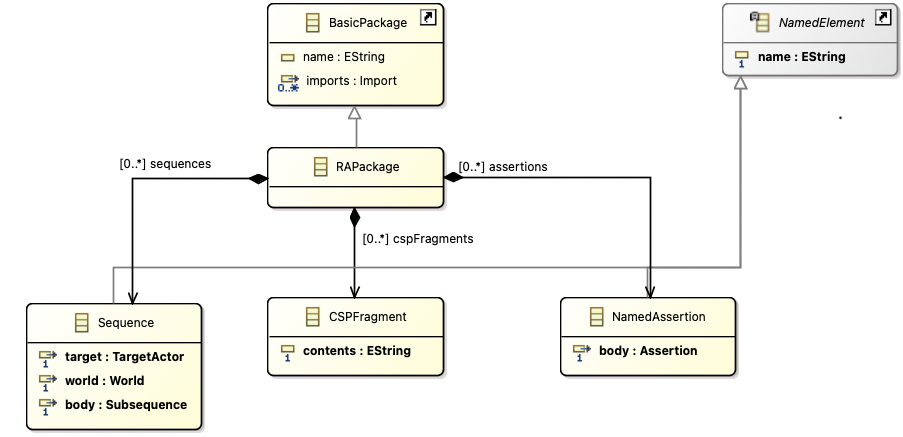
\includegraphics[width=.8\textwidth]{diagrams/top.png}
	\caption{Class diagram for the top of the \langname{} metamodel.}
	\label{fig:metamodel-top}
\end{figure}

\Cref{fig:metamodel-top} is the top-level metamodel diagram for \langname.

Each \langname{} script contains an \mrapackage,\footnote{\mrapackage{} stands
for `RoboStar Assertions package'; we use this name because \mrcpackage{} is
already used for RoboChart packages.}
which is a type of RoboStar \mbasicpackage.
Each \mrapackage{} can contain zero or more of each of these types of content:

\begin{itemize}
\item
	\msequence{}
	(\cref{sec:metamodel-sequences}):
	a sequence diagram;
\item
	\mcspfragment:
	a CSP fragment, currently not bound to a particular process
	\todo{this will change};
\item
	\mnamedassertion{}
	(\cref{sec:metamodel-assertions}):
	a named assertion, currently over sequence diagrams only
	\todo{more types of assertion will appear};
\end{itemize}

\todo{Elements might need to inherit from a common class and be stored in
the same list at some point.}


\section{Sequences, subsequences, and steps}\label{sec:metamodel-sequences}

\begin{figure}
	\centering
	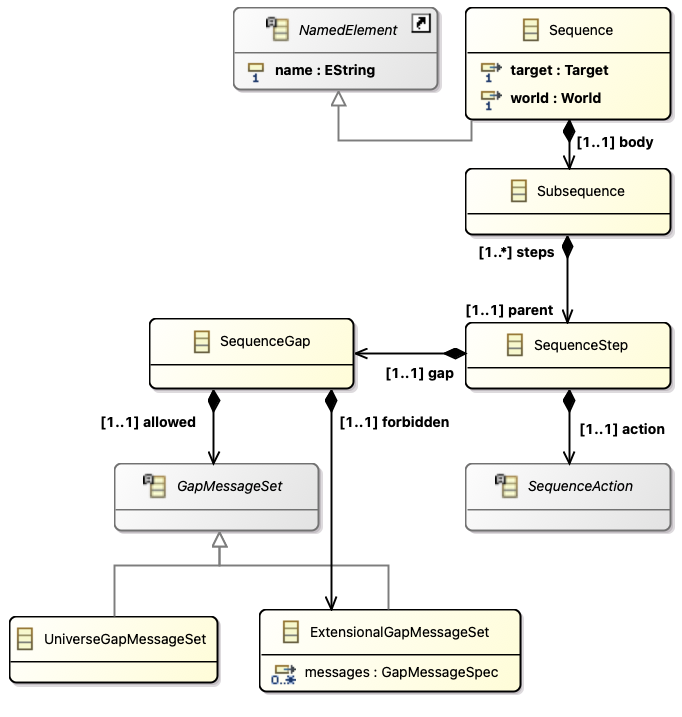
\includegraphics[width=\textwidth]{diagrams/sequences.png}
	\caption{Class diagram for the part of the \langname{} metamodel dealing with sequences.}
	\label{fig:metamodel-sequences}
\end{figure}

\Cref{fig:metamodel-sequences} depicts the part of the metamodel concerning
sequence diagrams.

\subsection{Sequences}

\begin{lstlisting}[style=Example]
sequence Example
  for module ModuleName as M,  // target actor (RoboChart module)
      world             as W   // world actor
{
	anything until end  // subsequence
}
\end{lstlisting}

A \msequence{} represents a single sequence diagram.  It is a \mnamedelement{}
that contains:

\begin{itemize}
\item
	a \msubsequence{} (\cref{ssec:metamodel-sequences-subsequences})
	containing the body of the diagram;
\item
	two \mactor s (\cref{sec:metamodel-actors}):
	a \mtargetactor{} (\cref{ssec:metamodel-actors-target})
	and a \mworld{} (\cref{ssec:metamodel-actors-world}).
\end{itemize}

\subsection{Subsequences}\label{ssec:metamodel-sequences-subsequences}

\begin{lstlisting}[style=Example]
{
	anything until operation O1() from M to W  // step
then
	operation O2() from M to W                 // step
then
	end                                        // step
}
\end{lstlisting}

A \msubsequence{} is a sequential composition of one or more \msequencestep s
(\cref{ssec:metamodel-sequences-steps}).
All \msequence s contain at least one \msubsequence{} at the top level, but
may contain multiple nested \msubsequence s introduced by constructs such as
\mloopaction s.

\subsection{Steps}\label{ssec:metamodel-sequences-steps}

\begin{lstlisting}[style=Example]
anything until             // gap
operation O() from M to W  // action
\end{lstlisting}

A \msequencestep{} is a single step in a \msubsequence.  It consists of a
\msequencegap{} (\cref{ssec:metamodel-sequences-gaps}) and a
\msequenceaction{} (\cref{sec:metamodel-sequences-actions}).

\subsection{Gaps}\label{ssec:metamodel-sequences-gaps}

\begin{lstlisting}[style=Example]
anything
	in     { operation O1() from M to W, operation O2() from M to W }  // allow set
	except { operation O2() from M to W }                              // forbid set

	// a universe set is implied for the allow set if 'in {..}' is omitted
	// an empty extensional set is implied for the forbidden set if 'except {..}' is omitted
until // only permits O1
\end{lstlisting}

A \msequencegap{} represents a condition on any communication\footnote{In PSCs,
this would correspond to \emph{intraMSG}s.} that can happen
\emph{before} a \msequenceaction.  
It contains two \mgapmessageset s: one specifying the messages
\emph{allowed} to pass inside the gap, and another specifying the messages
\emph{forbidden} to pass.\footnote{The \emph{forbidden} set is always an
\mextensionalgapmessageset, as any gap with a universal
\emph{forbidden} set would always be equivalent to one with an empty
\emph{allowed} set.
}

\paragraph{Gap message sets}

A \mgapmessageset{} is an expression of the set of messages allowed or forbidden
inside a \msequencegap.  There are two types of \mgapmessageset:

\begin{itemize}
\item
	a \muniversegapmessageset{} represents the universal set containing 
	all possible messages, and
	captures a lack of specific restriction on
	the \emph{allowed} set of a \msequencegap;
\item	
	an \mextensionalgapmessageset{} is a set (expressed as an unordered list) of
	zero or more \mgapmessagespec s, themselves
	a type of \mmessagespec{} (\cref{sec:metamodel-messages}).
\end{itemize}

There is not yet any meaningful extra data stored in
\mgapmessagespec s that is not present in \mmessagespec s, but this is subject
to change.


\subsection{Actions}\label{sec:metamodel-sequences-actions}

\begin{lstlisting}[style=Example]
operation O1() from M to W  // arrow action

loop L {
	operation O2() from M to W
}  // loop action (taking a subsequence)

end  // final action
\end{lstlisting}

A \msequenceaction{} is an explicit communication or control flow construct in a
\msubsequence.  There are currently three types of action: arrow, loop, and
final actions.

\paragraph{Arrow actions}

An \marrowaction\footnote{The name signifies both that the actions resemble
PSC \emph{arrowMSG} specifications, and also that they correspond to arrows in
the graphical syntax.} specifies one communication between \mactor s which is on
the sequence specified by the diagram.  Each \marrowaction{} wraps one
\marrowmessagespec{} (\cref{sec:metamodel-messages})
containing the specification proper.
\todo{Eventually these will bind arguments.}

\paragraph{Loop actions}

A \mloopaction{} is a \emph{named} infinite loop.  \todo{Breaking and perhaps
other forms of loop are forthcoming.}  Each \mloopaction{} contains one
\msubsequence{} of steps to repeat indefinitely.
\todo{If \mloopaction s could contain zero \msubsequence s, or \msubsequence s
could contain zero \msequencestep s, they could
explicitly capture deadlock, but currently so does \mfinalaction.}

\paragraph{Final actions}

A \mfinalaction{} represents the end of a sequence diagram, corresponding
to a point in time where the sequence target has either terminated or stopped
responding.  It primarily serves to allow a final \msequencegap{} to specify
any permitted communications after the behaviour explicitly specified by the
diagram has occurred.
\todo{Is the termination behaviour correct here?  Are there any useful
parallels between this and a hypothetical empty-bodied loop action?}


\section{Message specifications and topics}\label{sec:metamodel-messages}

\begin{figure}
	\centering
	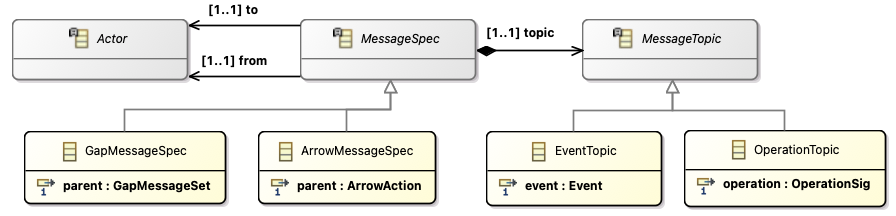
\includegraphics[width=.8\textwidth]{diagrams/messages.png}
	\caption{Class diagram for the part of the \langname{} metamodel dealing with messages.}
	\label{fig:metamodel-messages}
\end{figure}

\Cref{fig:metamodel-messages} depicts the part of the metamodel concerning
message specifications (`specs').

\subsection{Message specifications}

\begin{lstlisting}[style=Example]
operation O1() from M to W  // spec with operation topic, from actor M to actor W
event E        from W to M  // spec with event topic, from actor W to actor M
\end{lstlisting}

A \mmessagespec{} is a specification on the types of communication that can
happen during a gap (a \mgapmessagespec) or arrow (an \marrowmessagespec).\footnote{
This class distinction resembles that in PSCs betweeen intraMSGs and arrowMSGs,
respectively.}  Each \mmessagespec{} contains:

\begin{itemize}
\item
	references to two \mactor s, representing the \emph{to} and \emph{from}
	edges of the communication;
\item
	the \mmessagetopic{} (\cref{ssec:metamodel-messages-topics}) specifying
	the type of communication that the spec is capturing.
\end{itemize}

\subsection{Topics}\label{ssec:metamodel-messages-topics}

A \mmessagetopic{} identifies the specific type of communication in a
\mmessagespec{}.  There are currently two types of topic, corresponding to
RoboChart operations (\moperationmessagetopic) and events (\meventmessagetopic).
Each contains a reference to the signature of the respective construct.
Parameterised operations and events are not yet supported \todo{this will
change soon}.


\section{Actors}\label{sec:metamodel-actors}

\begin{figure}
	\centering
	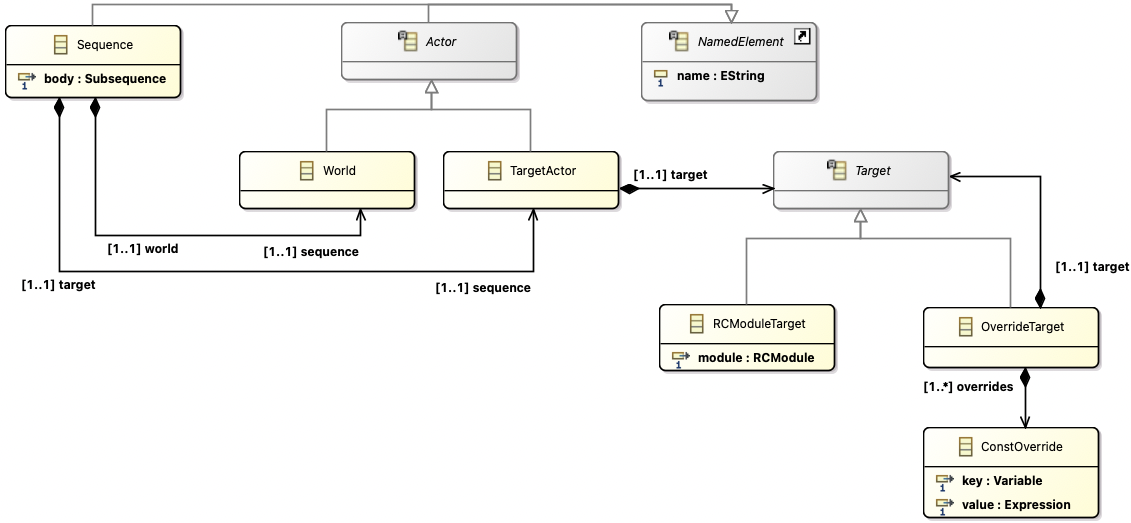
\includegraphics[width=\textwidth]{diagrams/actors.png}
	\caption{Class diagram for the part of the \langname{} metamodel dealing with actors.}
	\label{fig:metamodel-actors}
\end{figure}

\Cref{fig:metamodel-actors} depicts the part of the metamodel concerning
actors.

An \mactor{} is a named participant in a sequence.  The names can be used to
specify the direction of travel in \mmessagespec{}s.
As mentioned in
\cref{sec:metamodel-sequences}, there are always two actors
attached to a sequence: a \mtargetactor{} (\cref{ssec:metamodel-actors-target})
and a \mworld{} (\cref{ssec:metamodel-actors-world}).

\subsection{Targets and target actors}\label{ssec:metamodel-actors-target}

A \mtarget{} is an \emph{anonymous} specification of the part of a robotic
system that serves as the focus for a particular sequence diagram.  There are
presently two types of target, with more to appear later:

\begin{itemize}
\item
	a \mrcmoduletarget{} references a \mrcmodule;
\item
	an \moverridetarget{} wraps another \mtarget, overriding constant
	definitions.
\end{itemize}

A \mtargetactor{} wraps a \mtarget{} with a name, making it suitable as an
\mactor.  The separation between \mtarget{} and \mtargetactor{} allows for
patterns like \moverridetarget{} to exist without introducing unnecessary names.

\subsection{Worlds}\label{ssec:metamodel-actors-world}

A \mworld{} is an \mactor{} that represents the `world' outside a sequence
diagram's target.  \mworld s do not contain any data.

\section{Assertions}\label{sec:metamodel-assertions}

\begin{figure}
	\centering
	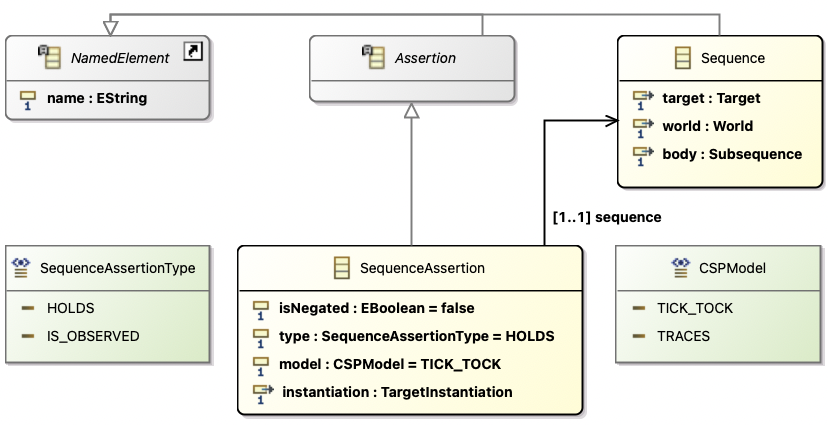
\includegraphics[width=0.7\textwidth]{diagrams/assertions.png}
	\caption{Class diagram for the part of the \langname{} metamodel dealing with assertions.}
	\label{fig:metamodel-assertions}
\end{figure}

\Cref{fig:metamodel-assertions} depicts the part of the metamodel concerning
assertions.

An \massertion{} is an \emph{anonymous} assertion statement.  Currently, there is
only one type of assertion: a \msequenceassertion{}.  \todo{This will change
when merging with the existing language, if not sooner.}

A \msequenceassertion{} is an assertion about a particular \msequence{} with
respect to a particular \mtarget.  By default, the \mtarget{} is that of the
\msequence{}. \todo{This isn't yet explicit in the metamodel.}  Specifying a
custom \mtarget{} as part of the assertion instead makes the assertion refer
to that target.

The specific sequence assertion type comes from the \msequenceassertiontype:
either `sequence holds on target' (refinement), or `sequence is observed on
target' (reverse refinement).  The assertion can be negated.  The choice of
\mcspmodel{} affects how the assertion is checked with CSP tools such as FDR
\todo{the models are incorrect in respect to timed assertions; I haven't yet
decided the best approach to allow the appropriate models in both timed and
untimed modes.  Currently, everything is untimed, and this too will change.}

A \mnamedassertion{} binds an \massertion{} to a name.


\chapter{Textual syntax}\label{cha:textual}
This section describes the textual syntax of \langname{} sequence
diagrams.  This syntax primarily uses controlled English, with
some use of braces and symbols to impose further structure.

\todo{TODO}

%%% Local Variables:
%%% mode: latex
%%% TeX-master: "../robocert"
%%% End:


\chapter{Graphical syntax}\label{cha:graphical}
This section describes the graphical syntax of \langname.

\todo{TODO}

\section{Principles}

\todo{These need work.}

\begin{itemize}
\item Where possible, we draw graphical cues from existing notations.
  This simplifies the uptake of the language for practitioners
  familiar with those notations.  Generally, cues for features come
  from whichever language is identified as the main inspiration in
  \cref{sec:metamodel-features}.
\item Where graphical elements attach to one side of a sequence diagram,
  we choose the side that is most relevant to that element.  For instance:
  \begin{itemize}
  \item \msequencegap s on \marrowaction s attach to whichever
    side is the source of the arrow, to emphasise that the gap modifies
    the act of \emph{sending} the message \todo{I'm not sure this is convincing};
  \item \msequencegap s on \mfinalaction s attach to the \mtarget{} end,
    since the \mfinalaction{} is similar to a message from the \mtarget{} to
    the \mworld{} specifying the \mtarget{} is finished.
  \end{itemize}
\end{itemize}

%%% Local Variables:
%%% mode: latex
%%% TeX-master: "robocert"
%%% End:

\part{Well-formedness and Semantics}

\chapter{Well-formedness}\label{cha:wf}
%!TEX root=./robocert.tex

This section contains well-formedness rules for the metamodel in
\cref{cha:metamodel}.

\todo{These are informal at the moment.}

\section{Packages}\label{sec:wf-top}

These rules concern the definitions in \cref{sec:metamodel-top}.

\section{Sequences}\label{sec:wf-sequences}

These rules concern the definitions in \cref{sec:metamodel-sequences}.

\section{Actions}\label{sec:wf-actions}

These rules concern the definitions in \cref{sec:metamodel-actions}.

\begin{enumerate}
\item
	A \msequence{} \rfcmustnot{} contain more than one \mfinalaction.
\item
	Any \mfinalaction{} \rfcmust{} be the last action in the topmost
	\msubsequence{} of a \msequence.
\end{enumerate}

\section{Messages}\label{sec:wf-messages}

These rules concern the definitions in \cref{sec:metamodel-messages}.

\subsection{\mmessagespec}

\paragraph{Actors}

\begin{enumerate}
\item
	Exactly one of the from-- and to-actors of a message spec \rfcmust{} 
	be a \mtarget.
	\todo{unenforced}
\item
	Exactly one of the from-- and to-actors of a message spec \rfcmust{} 
	be a \mworld.
	\todo{unenforced}
\end{enumerate}

\paragraph{Arguments}

\begin{enumerate}
\item
	\mrestargument{} \rfcmustnot{} appear anywhere other than as the last
	argument in the list.
	\todo{unenforced}
\item
	Argument lists \rfcmust{} either end in a \mrestargument, or
	contain exactly as many arguments as the \mmessagetopic{} of the spec
	has parameters.  (An \meventtopic{} is considered to have 1 parameter
	if typed, and 0 otherwise.)
	\todo{unenforced}
\item
	Argument lists \rfcmustnot{} contain more
	arguments than the \mmessagetopic{} of the spec has parameters.
	As this includes \mrestargument, this means that \mrestargument{} cannot
	appear if all parameters already have arguments.
	\todo{unenforced}
\item
	\mexpressionargument s \rfcshould{} be literals.  This is a temporary
	limitation, and will be lifted when the CSP generator improves.
	\todo{unenforced}
\end{enumerate}

\section{Actors}\label{sec:wf-actors}

These rules concern the definitions in \cref{sec:metamodel-actors}.

\section{Assertions}\label{sec:wf-assertions}

These rules concern the definitions in \cref{sec:metamodel-assertions}.


\chapter{Semantics}\label{cha:semantics}
%!TEX root=./robocert.tex

% Target language colouration
\newcommand{\tlang}[1]{\textcolor{TColor}{\boxed{#1}}}
% Object language colouration (nested inside target language)
\newcommand{\olang}[1]{\boxed{\textcolor{ZedColor}{#1}}}

\newcommand{\tockcsp}{\emph{tock}-CSP}
\newcommand{\cspm}{CSP\(_\text{M}\)}

\newcommand{\defeq}{\mathbin{\overset{\text{def}}=}}
% CSP operators
\newcommand{\interrupt}{\mathbin{\triangle}}
\newcommand{\cspnsop}{\mathbin{\!:\!:\!}}
% CSP keywords/processes
\newcommand{\cspkw}[1]{\operatorname{\mathbf{#1}}}
\newcommand{\runproc}[1]{\cspkw{Run}\left(#1\right)}
\newcommand{\events}{\cspkw{Events}}

%
% Metasyntactic variables
%
\newcommand{\acontext}{c}
\newcommand{\anexpr}{e}
\newcommand{\avar}{v}
% Top-level
\newcommand{\apkg}{P}
\newcommand{\acsp}{f}
% Sequences
\newcommand{\aseq}{\sigma}
\newcommand{\asseq}{q}
\newcommand{\astep}{s}
\newcommand{\agap}{g}
% Actions
\newcommand{\anaction}{a}
\newcommand{\anarrow}{\rho}
\newcommand{\aloop}{l}
% Messages
\newcommand{\amspec}{m}
\newcommand{\amsgset}{M}
\newcommand{\aumsgset}{\amsgset_{\universe}}
\newcommand{\anemsgset}{\amsgset_{e}}
\newcommand{\armsgset}{\amsgset_{r}}
\newcommand{\anevent}{\epsilon}
\newcommand{\anop}{o}
% - Arguments
\newcommand{\anarg}{x}
\newcommand{\anexprarg}{\anarg_\anexpr}
\newcommand{\arestarg}{\anarg_r}
\newcommand{\anarglist}{\mathbf{x}}
% Actors
\newcommand{\atarget}{t}
\newcommand{\aninst}{\phi}
\newcommand{\aworld}{w}
% Assertions
\newcommand{\anasst}{\alpha}
\newcommand{\asasst}{\alpha_s}
\newcommand{\amodel}{\mathcal{M}}

% External semantics
\newcommand{\exprsema}[2]{\sema{#1}{expr}_{(#2)}}

\newcommand{\sema}[2]{\llbracket #1 \rrbracket^{\mathsf{#2}}}
\newcommand{\pkgsema}[1]{\sema{#1}{pkg}}
\newcommand{\cspsema}[1]{\sema{#1}{csp}}
\newcommand{\stepsema}[1]{\sema{#1}{step}}
\newcommand{\gapsema}[2]{\sema{#1}{gap}_{(#2)}}
\newcommand{\actsema}[1]{\sema{#1}{act}}
\newcommand{\mspecsema}[2]{\sema{#1}{mspec}_{\text{#2}}}
\newcommand{\pmspecsema}[1]{\mspecsema{#1}{prefix}}
\newcommand{\emspecsema}[1]{\mspecsema{#1}{events}}
\newcommand{\arglistsema}[2]{\sema{#1}{args}_{(#2)}}
\newcommand{\loopsema}[1]{\sema{#1}{loop}}
\newcommand{\msgsetsema}[1]{\sema{#1}{mset}}
\newcommand{\seqsema}[1]{\sema{#1}{seq}}
\newcommand{\sseqsema}[1]{\sema{#1}{sseq}}
\newcommand{\asstsema}[1]{\sema{#1}{asst}}

\newcommand{\targetsema}[2]{\sema{#1}{target}_{(#2)}}

\newcommand{\funcname}[1]{\ensuremath{\mathsf{#1}}}
\newcommand{\eventsOf}[1]{\funcname{events}(#1)}
\newcommand{\seqnameOf}[1]{\funcname{seqName}(#1)}
\newcommand{\ctargetnameOf}[1]{\funcname{ctargetName}(#1)}
\newcommand{\otargetnameOf}[1]{\funcname{otargetName}(#1)}

\newcommand{\field}[2]{#1.\funcname{#2}}

This chapter formally captures the semantics of \langname{} in terms of its
target languages:

\begin{itemize}
\item
	\tockcsp~(\cref{sec:semantics-tockcsp});
\item
	\todo{PRISM};
\item
	\todo{Isabelle/UTP?}.
\end{itemize}

Each semantics captures \massertion s as the top-level definition, with all
objects reachable from the assertions translated in-line.  As a
consequence, we do not capture organisational details such as \mrapackage s,
or any distinction between references to objects and their definitions.

\section{How to read this section}

\begin{table}
  \centering

  \begin{tabular}{p{2em}p{10.5em}}
    \toprule
    \thead{Var.}
    & \thead{Type}
    \\
    \midrule
    \multicolumn{2}{l}{\tsubhead{\robochart{} imports}}
    \\
    \(\avar\) & \mvariable
    \\
    \(\anexpr\) & \mexpression
    \\
    \bottomrule
  \end{tabular}
  \begin{tabular}{p{2em}p{10.5em}}
    \toprule
    \thead{Var.}
    & \thead{Type}
    \\
    \midrule
    \multicolumn{2}{l}{\tsubhead{Packages (\cref{sec:metamodel-top})}}
    \\
    \(\apkg\) & \mrapackage
    \\
    \(\acsp\) & \mcspfragment
    \\
    \midrule
    \multicolumn{2}{l}{\tsubhead{Sequences (\cref{sec:metamodel-sequences})}}
    \\
    \(\aseq\) & \msequence
    \\
    \(\asseq\) & \msubsequence
    \\
    \(\astep\) & \msequencestep
    \\
    \(\agap\) & \msequencegap
    \\
    \midrule
    \multicolumn{2}{l}{\tsubhead{Steps (\cref{sec:metamodel-steps})}}
    \\
    \(\aloop\) & \mloopstep
    \\
    \midrule
    \multicolumn{2}{l}{\tsubhead{Actions (\cref{sec:metamodel-actions})}}
    \\
    \(\anaction\) & \msequenceaction
    \\
    \(\anarrow\) & \marrowaction
    \\
    \(\bot\) & \mfinalaction
    \\
    \\
    \\
    \\
    \\
    \bottomrule
  \end{tabular}
  \begin{tabular}{p{2em}p{10.5em}}
    \toprule
    \thead{Var.}
    & \thead{Type}
    \\
    \midrule
    \multicolumn{2}{l}{\tsubhead{Messages (\cref{sec:metamodel-messages})}}
    \\
    \(\amspec\) & \mmessagespec
    \\
    \(\amsgset\) & \mmessageset
    \\
    \(\aumsgset\) & \muniversemessageset
    \\
    \(\anemsgset\) & \mextensionalmessageset
    \\
    \(\armsgset\) & \mrefmessageset
    \\
    \(\anarg\) & \margument
    \\
    \(\anexprarg\) & \mexpressionargument
    \\
    \(\arestarg\) & \mrestargument
    \\
    \midrule
    \multicolumn{2}{l}{\tsubhead{Actors (\cref{sec:metamodel-actors})}}
    \\
    \(\atarget\) & \mtarget
    \\
    \(\aworld\) & \mworld
    \\
    \(\aninst\) & \mtargetinstantiation
    \\
    \midrule
    \multicolumn{2}{l}{\tsubhead{Assertions (\cref{sec:metamodel-assertions})}}
    \\
    \(\anasst\) & \massertion
    \\
    \(\asasst\) & \msequenceassertion
    \\
    \(\amodel\) & \mcspmodel	
    \\
    \bottomrule
  \end{tabular}
  
  \caption{Metasyntactic variables.}
  \label{tab:metasyntactic-variables}
\end{table}

The semantics treatments in this section take the form of rewrite rules from
the abstract syntax in \cref{cha:metamodel} to some object language (for
instance, \tockcsp).
For conciseness, we use a meta-language based on the Z notation.
We also use the following notational conventions:

\begin{itemize}
\item
	\(\sema{-}{name}\) denotes a main semantic rule;
\item
	\(\funcname{name}()\) denotes auxiliary semantic functions;
\item
	\(\field{x}{name}\) denotes a field of the metamodel object \(x\);
\item
	\tlang{\text{boxed shaded text}} denotes a construct from the object
	language; outside such text, or \tlang{\olang{\text{inside nested boxes}}},
	assume use of the meta-language.  For example, consider the \tockcsp{}
	construct:
	\[\tlang{
		\runproc{\olang{\gapsema{\field{\astep}{gap}}{\field{\astep}{action}}}}
		\interrupt \olang{\actsema{\field{\astep}{action}}}
	}\]
	Here, \(\runproc{}\) and \(\interrupt\) are part of \tockcsp, while
	\(\actsema{\field{\astep}{action}}\) is an semantic operation on the
	\langname{} metamodel.
\item
	variables in the meta-language have an implicit metamodel type
	corresponding to one of the metasyntactic variables in
	\cref{tab:metasyntactic-variables}.
\end{itemize}

\section{Dependencies on the \robochart{} semantics}

\newcommand{\targetProcess}[1]{\ensuremath{\funcname{targetProcess}\left(#1\right)}}
\newcommand{\targetParams}[1]{\ensuremath{\funcname{targetParams}\left(#1\right)}}
\newcommand{\constName}[1]{\ensuremath{\funcname{constName}\left(#1\right)}}

\todo{this may need to move to the \tockcsp{} section eventually}

Each semantics treatment in this section assumes the existence of a compatible
semantics over \robochart.  Specifically, we assume the following rules and
functions are available, or can be derived, from such a semantics:

\begin{itemize}
\item
	let \targetProcess{-} map a target to the parametric
	process exposed by the relevant \tockcsp{} semantics (for instance,
	we delegate to the \robochart{} semantics for the underlying
	\mrcmodule{} of a \mrcmoduletarget);
	\todo{doesn't account for the ID parameter in certain target
	processes};
\item
	let \targetParams{-} map a target to the sequence of
	constants in its parameterisation;
\item
	let \constName{-} map a constant to its name in the \robochart{}
	instantiations file;
\item
	let \(\exprsema{\anexpr}{\acontext}\) be the expression semantics of 
	\(\anexpr\) in the context \(\acontext\).  The expression semantics
	is external to this semantics, but is largely that of Z.
\end{itemize}

\section{\tockcsp{} semantics}\label{sec:semantics-tockcsp}
%!TEX root=../robocert.tex

This section introduces a \tockcsp{} semantics for \langname.
\todo{Need to make sure it's actually \tockcsp, not CSP.}
This semantics is inspired by that of Lima et al. on the CML semantics of
UML sequence diagrams.

The behaviour of the \langname{} generator is expected to conform to
this semantics, except that:

\begin{itemize}
\item
  The generator targets \cspm{} instead of CSP, and so \emph{may}
  use semantically equivalent \cspm{} constructs where the CSP equivalents
  are missing or not idiomatic;
\item
  The generator \emph{must} \todo{not yet but eventually} wrap processes in
  timed sections and prioritisations to achieve the appropriate \tockcsp{} behaviours of
  CSP operators;
\item
  The generator \emph{may} perform semantics-preserving optimisations,
  such as substituting \(P\) for \(\tlang{\Stop \interrupt \olang{P}}\).
\end{itemize}

\todo{Some of the definitions are very loosely typed (as they are expanding from
a metamodel to textual snippets of something halfway between \tockcsp{} and
\cspm), and it'd be nice to fix that and/or give explicit result types.}

\subsection{Assertions}

The definitions here correspond to \cref{sec:metamodel-assertions}.

\begin{definition}[\massertion]

\newcommand{\refop}[3]{\mathbin{\odot_{#1}^{(#2, #3)}}}

The only type of assertion so far is \msequenceassertion.  The semantics of a
\msequenceassertion{} relates the \msequence{} of the assertion to the
\mtarget{} of the assertion.
%
\begin{align*}
	\asstsema{\asasst}
\quad\defeq\quad&
	\seqnameOf{\field{\asasst}{sequence}}
	\;
	\refop{\field{\asasst}{model}}{\field{\asasst}{isNegated}}{\field{\asasst}{type}}
	\;
	\targetsema{\field{\field{\asasst}{sequence}}{target}}{\field{\asasst}{instantiation}}
\end{align*}

The exact refinement operator depends on the assertion type and negation:
%
\begin{align*}
	\refop{\amodel}{\true}{\mathsf{holds}}
\quad\defeq\quad&
	\tlang{\sqsubseteq_{\olang{\amodel}}}
&
	\refop{\amodel}{\false}{\mathsf{holds}}
\quad\defeq\quad&
	\tlang{\not\sqsubseteq_{\olang{\amodel}}}
\\
	\refop{\amodel}{\true}{\mathsf{isObserved}}
\quad\defeq\quad&
	\tlang{\sqsupseteq_{\olang{\amodel}}}
&
	\refop{\amodel}{\false}{\mathsf{isObserved}}
\quad\defeq\quad&
	\tlang{\not\sqsupseteq_{\olang{\amodel}}}
\\
\end{align*}
\end{definition}


\subsection{Sequences}\label{ssec:semantics-tockcsp-sequences}

The definitions here correspond to \cref{sec:metamodel-sequences}.

\begin{definition}[\msequence]

The semantics of a \msequence{} is that of its subsequence
\todo{eventually, in parallel with its memory}.
%
\begin{align*}
	\seqsema{\aseq}
\quad\defeq\quad&	
	\sseqsema{\field{\aseq}{body}}
\end{align*}

\end{definition}

\begin{definition}[\msubsequence]

The semantics of a \msubsequence{} is a sequential composition of that of its steps.
%
\begin{align*}
	\sseqsema{\asseq}
	\quad\defeq\quad&	
	\funcname{steps}(\field{\asseq}{body})
\\
	\funcname{steps}(\langle \astep_1, \dotsc, \astep_n \rangle)
	\quad\defeq\quad&	
	\tlang{
	\olang{\stepsema{\astep_1}}
	\circseq
	\olang{\dotso}
	\circseq
	\olang{\stepsema{\astep_n}}
	}
\end{align*}

\end{definition}

\todo{\msequencestep}

\begin{definition}[\mactionstep]

The semantics of a \mactionstep{} is an unbounded loop over the events of its
\msequencegap, interrupted by the \msequenceaction.\footnote{Note that the semantics of the gap depends
on the action.  This is because, as seen in \(\gapsema{\agap}{\anaction}\),
the events on which the action can interrupt the
gap must be removed from the events of the gap to ensure the interrupt has the
expected semantics.}
%
\begin{align*}
	\stepsema{\astep}
\quad\defeq\quad&	
	\tlang{
		\runproc{\olang{\gapsema{\field{\astep}{gap}}{\field{\astep}{action}}}}
		\interrupt \olang{\actsema{\field{\astep}{action}}}
	}
\end{align*}
\end{definition}

\begin{definition}[\msequencegap]
	The semantics of a \msequencegap{} is the CSP event set corresponding to
	the difference between the \emph{allowed} set and any events
	the action following the gap can initially communicate.
%
\begin{align*}
	\gapsema{
		\agap
	}{\anaction}
\quad\defeq\quad&
\tlang{
	\olang{\msgsetsema{\field{\agap}{allowed}}}
	\setminus
	\olang{\eventsOf{\anaction}}
}
\end{align*}
\end{definition}

\begin{definition}[CSP event sets]
For now, the event set of an action is the prefix of an arrow action, or
the empty set for any other actions.  This will change when the prefix becomes
inexpressible as an event set.
%
\begin{align*}
	\eventsOf{\anarrow}
\quad\defeq\quad&
	\tlang{\Set{\olang{\emspecsema{\anarrow}}}}
	\tag{arrow}
\\
	\eventsOf{\anaction}
\quad\defeq\quad&
	\tlang{\emptyset}
	\tag{anything else}
\end{align*}
\end{definition}

\subsection{Actions}\label{ssec:semantics-tockcsp-actions}

The definitions here correspond to \cref{sec:metamodel-actions}.

\begin{definition}[\msequenceaction]

The semantics of an arrow action is the semantics of its arrow as a CSP prefix,
prefixing termination.  The semantics of a loop delegates to a separate rule
over its label and subsequence.
%
\begin{align*}
	\actsema{\anarrow}
\quad\defeq\quad&
	\tlang{
	\left(
	\olang{\pmspecsema{\anarrow}}
	\then
	\Skip
	\right)
	}
	\tag{arrow action}
\\
	\actsema{\aloop}
\quad\defeq\quad&
	\loopsema{\aloop}
\tag{loop action}
\\
	\actsema{\bot}
\quad\defeq\quad&
	\tlang{\Skip}
\tag{final action}
\end{align*}

\end{definition}

\newcommand{\iloop}[1]{\text{Loop}(#1)}
\newcommand{\nloop}[1]{\text{Loop}_\sqcap(#1)}
\newcommand{\dloop}[2]{\text{Loop}_d(#1, #2)}
\newcommand{\lloop}[2]{\text{Loop}_l(#1, #2)}
\newcommand{\uloop}[2]{\text{Loop}_u(#1, #2)}
\newcommand{\rloop}[3]{\text{Loop}_r(#1, #2, #3)}

\begin{definition}[\mloopstep]  
For now, the semantics of a loop is that of the loop
subsequence hoisted into an auxiliary loop-running process (defined
below).
\todo{define the symbols used here}
%
\begin{align*}
  \loopsema{\aloop}
  \quad\defeq\quad
  &
    \funcname{runner}(\field{\aloop}{bound}, \sseqsema{\field{\aloop}{body}})
  \\
  \funcname{runner}(\infty, P)
  \quad\defeq\quad
  & \tlang{\iloop{\olang{P}}}
    \tag{infinite loops}
  \\
  \funcname{runner}(n, P)
  \quad\defeq\quad
  & \tlang{\dloop{\olang{\exprsema{n}{\emptyset}}}{\olang{P}}}
    \tag{definite-bound loops}
  \\
  \funcname{runner}((l, \ast), P)
  \quad\defeq\quad
  & \tlang{\lloop{\olang{\exprsema{l}{\emptyset}}}{\olang{P}}}
    \tag{lower-bound loops}
  \\
  \funcname{runner}((l, u), P)
  \quad\defeq\quad
  & \tlang{\rloop{\olang{\exprsema{l}{\emptyset}}}{\olang{\exprsema{u}{\emptyset}}}{\olang{P}}}
    \tag{range-bound loops}
  \\  
\end{align*}

\end{definition}

\begin{definition}[Auxiliary loop processes]

We can define the loop processes used above in CSP as follows:
%
\begin{align*}
  \iloop{P}
  \quad\defeq\quad
  & P \circseq \iloop{P}
    \tag{infinite}
  \\
  \nloop{P}
  \quad\defeq\quad
  & \Skip \sqcap \left(P \circseq \nloop{P}\right)
    \tag{nondeterministic}
  \\  
  \dloop{n}{P}
  \quad\defeq\quad
  & \Skip \triangleleft n \leq 0 \triangleright \left(P \circseq \dloop{n-1}{P}\right)
    \tag{definite}
  \\
  \uloop{n}{P}
  \quad\defeq\quad
  & \Skip \triangleleft n \leq 0 \triangleright \left(\Skip \sqcap \left(P \circseq \uloop{n-1}{P}\right)\right)
    \tag{upper-bound}
  \\
  \lloop{n}{P}
  \quad\defeq\quad
  & \dloop{n}{P} \circseq \nloop{P}
    \tag{lower-bound}
  \\
  \rloop{l}{u}{P}
  \quad\defeq\quad
  & \lloop{l}{P} \circseq \uloop{u - l}{P}
    \tag{range}
  \\
\end{align*}
\end{definition}

\subsection{Messages}\label{ssec:semantics-tockcsp-messages}

The definitions here correspond to \cref{sec:metamodel-messages}.

\begin{definition}[\mmessageset]

  The semantics of a message set is the universal event set for \muniversemessageset s;
  the expansion of the given \mgapmessagespec s for \mextensionalmessageset s;
  the semantics of the referred-to set for \mrefmessageset s;
  and the semantics of the referred-to set operator for \mbinarymessageset s.
%
\begin{align*}
  \msgsetsema{\aumsgset}
  \quad\defeq\quad
  &
    \tlang{\events}
    \tag{universe}
  \\
  \intertext{\todo{The meta/object language distinction is messy here
  and I'm not sure how to handle it.}}
  \msgsetsema{\anemsgset}
  \quad\defeq\quad
  &
    \tlang{
    \bigcup
    \olang{
    \Set{
    \emspecsema{\amspec} | \amspec \in \field{\anemsgset}{messages}
    }
    }
    }
    \tag{extensional}
  \\
  \msgsetsema{\armsgset}
  \quad\defeq\quad
  &
    \msgsetsema{\field{\field{\armsgset}{set}}{set}}
    \tag{reference}
  \\
  \msgsetsema{\amsgset_l \odot \amsgset_r}
  \quad\defeq\quad
  &
  \tlang{
    \olang{\msgsetsema{\amsgset_l}}
    \odot
    \olang{\msgsetsema{\amsgset_r}}
    \tag{binary-operator}
  }
\end{align*}
\end{definition}

There are two distinct semantic rules for \mmessagespec s.  One is used whenever
we expand the \mmessagespec{} into an event set, and handles `rest' arguments
by implicitly quantifying over the missing parameters.  The other is used when
expanding to a prefix, and introduces explicit discards for the missing
parameters.  \todo{The two forms will diverge further when we introduce
parameter binding.}

\begin{definition}[\mmessagespec{} as an event set]

We expand \mmessagespec s into event-set form in two stages: expanding
any non-`rest' arguments with \funcname{withArgs}, then expanding the channel
reference using \funcname{msgChan}.
%
\begin{align*}
	\emspecsema{\amspec}
\quad\defeq\quad&
\funcname{withArgs}\left(\field{\amspec}{arguments}, \amspec\right)
\\
	\funcname{withArgs}\left(\amspec, \anarglist\cat\langle\anexprarg\rangle\right)
\quad\defeq\quad&
\tlang{
	\olang{\funcname{withArgs}\left(\amspec, \anarglist\right)}
	!\olang{\exprsema{\anexprarg}{\amspec}}
}
\tag{expression argument}
\\
	\funcname{withArgs}\left(\amspec, \anarglist\cat\langle\arestarg\rangle\right)
\quad\defeq\quad&
	\funcname{withArgs}\left(\amspec, \anarglist\right)
\tag{rest argument}
\\
	\funcname{withArgs}\left(\amspec, \langle\rangle\right)
\quad\defeq\quad&
	\funcname{msgChan}\left(\amspec\right)
\tag{end of arguments}
\end{align*}
The expansion of the message channel
depends on the message topic
and, for certain topics, the direction (inbound from world to target, or
outbound from target to world).
\newcommand{\nsOf}[1]{\mathsf{ns}(#1)}
\newcommand{\targetOf}[2]{\mathsf{target}(#1,#2)}
\newcommand{\topicOf}[3]{\mathsf{topic}(#1,#2,#3)}
%
\begin{align*}
	\funcname{msgChan}(\amspec)
\quad\defeq\quad&
\tlang{
	\olang{\nsOf{\targetOf{\field{\amspec}{from}}{\field{\amspec}{to}}}}
	{}\cspnsop{}
	\olang{\topicOf{\field{\amspec}{topic}}{\field{\amspec}{from}}{\field{\amspec}{to}}}
}
\\
	\targetOf{\aworld}{\atarget}
\quad\defeq\quad&
	\targetOf{\atarget}{\aworld}
	\quad\defeq\quad
	\atarget
\\
	\topicOf{\anop}{\atarget}{\aworld}
\quad\defeq\quad&
\tlang{
	\olang{\field{\anop}{name}}\text{Call}
}
\tag{operation; always outbound}
\\
	\topicOf{\anevent}{\aworld}{\atarget}
\quad\defeq\quad&
	\tlang{\olang{\field{\anevent}{name}}\text{.in}}
\tag{inbound event}
\\
	\topicOf{\anevent}{\atarget}{\aworld}
\quad\defeq\quad&
	\tlang{\olang{\field{\anevent}{name}}\text{.out}}
\tag{outbound event}
\end{align*}
\end{definition}

\newcommand{\paramsOf}[1]{\funcname{params}(#1)}
\newcommand{\beforeRest}[1]{\funcname{beforeRest}(#1)}

\begin{definition}[\mmessagespec{} as a prefix]

To expand a \mmessagespec{} into a prefix, we take the event set expansion and
\todo{for now} \emph{pad} it with wildcard inputs for each topic parameter
left unmatched at the point of any \mrestargument.
%
\begin{align*}
	\pmspecsema{\amspec}
\quad\defeq\quad&
	\funcname{pad}\left(\emspecsema{\amspec}, \funcname{padding}(\amspec)\right)
\\
	\funcname{pad}(x, 0)
\quad\defeq\quad&
	x
\tag{base case}
\\
	\funcname{pad}(x, n)
\quad\defeq\quad&
\tlang{
	\olang{\funcname{pad}(x, n-1)}?\_
}
\tag{inductive case}
\\
	\funcname{padding}(\amspec)
\quad\defeq\quad&
	\#(\paramsOf{\field{\amspec}{topic}}) - \beforeRest{\field{\amspec}{arguments}}
\\
	\beforeRest{\langle\rangle}
\quad\defeq\quad&
	0
\tag{base case}
\\
	\beforeRest{\langle \arestarg \rangle \cat \anarglist}
\quad\defeq\quad&
	0
\tag{rest argument}
\\
	\beforeRest{\langle \anarg \rangle \cat \anarglist}
\quad\defeq\quad&
	1 + \beforeRest{\anarglist}
\tag{non-rest argument}
\end{align*}
\end{definition}

\subsection{Actors}\label{ssec:semantics-tockcsp-actors}

The definitions here correspond to \cref{sec:metamodel-actors}.


\begin{definition}[\mtarget]

The semantics of a target is the parametric process generated for that
target by the relevant external semantics, with constant parameters instantiated
as follows:

\begin{itemize}
\item
	if the constant is bound in the assertion's \mtargetinstantiation{}
	(passed to the semantics as \(\aninst\)), use the bound expression; else
\item
	if the constant is bound in the target's \mtargetinstantiation, use
	the bound expression; else
\item
	use the \(\funcname{constName}\) of the constant, under the assumption
	that it will later bind to a fallback instantiation for the constant.
\end{itemize}
%
\begin{align*}
	\targetsema{\atarget}{\aninst}
\quad\defeq\quad&
\tlang{
	\olang{\funcname{targetProcess}(\atarget)}
	\left(
		\olang{\exprsema{-}{\atarget}\ \circ\ \funcname{instantiate}(\aninst)\ \circ\ \funcname{targetParams}(\atarget)}
	\right)
}
\\
	\funcname{instantiate}(\aninst, \atarget)
\quad\defeq\quad&
	\funcname{constName}
	\oplus
	\field{\field{\atarget}{instantiation}}{constants}
	\oplus
	\field{\aninst}{constants}
\end{align*}
\end{definition}


%%% Local Variables:
%%% mode: latex
%%% TeX-master: "../robocert"
%%% End:


%%% Local Variables:
%%% mode: latex
%%% TeX-master: "robocert"
%%% End:


\appendix

\stopcontents

\chapter*{Credits}\label{cha:credits}
{\it
\noindent {\LaTeX\ style based on the The Legrand Orange Book Template
by Mathias Legrand and Vel from
\href{www.latextemplates.com}{LaTeXTemplates.com}. Licensed under
\href{http://creativecommons.org/licenses/by-nc-sa/3.0/}{CC BY-NC-SA
3.0}.}\\

\chapter*{Bibliography}
\addcontentsline{toc}{chapter}{\textcolor{ocre}{Bibliography}}
\printbibliography[heading=bibempty]

\end{document}